\section{Results}
\label{sec3:results}


In this section we present the results of our experiments\footnote{\href{https://youtu.be/gXf2Chu4L9A}{\color{blue}\textbf{https://youtu.be/gXf2Chu4L9A}} directs to a video overview of our experiments.} and indicate statistical significance under the Mann-Whitney $U$ test where applicable. 




\subsection*{Random search.}


\begin{figure}[t]
% \hspace{-0.4cm}
\centering
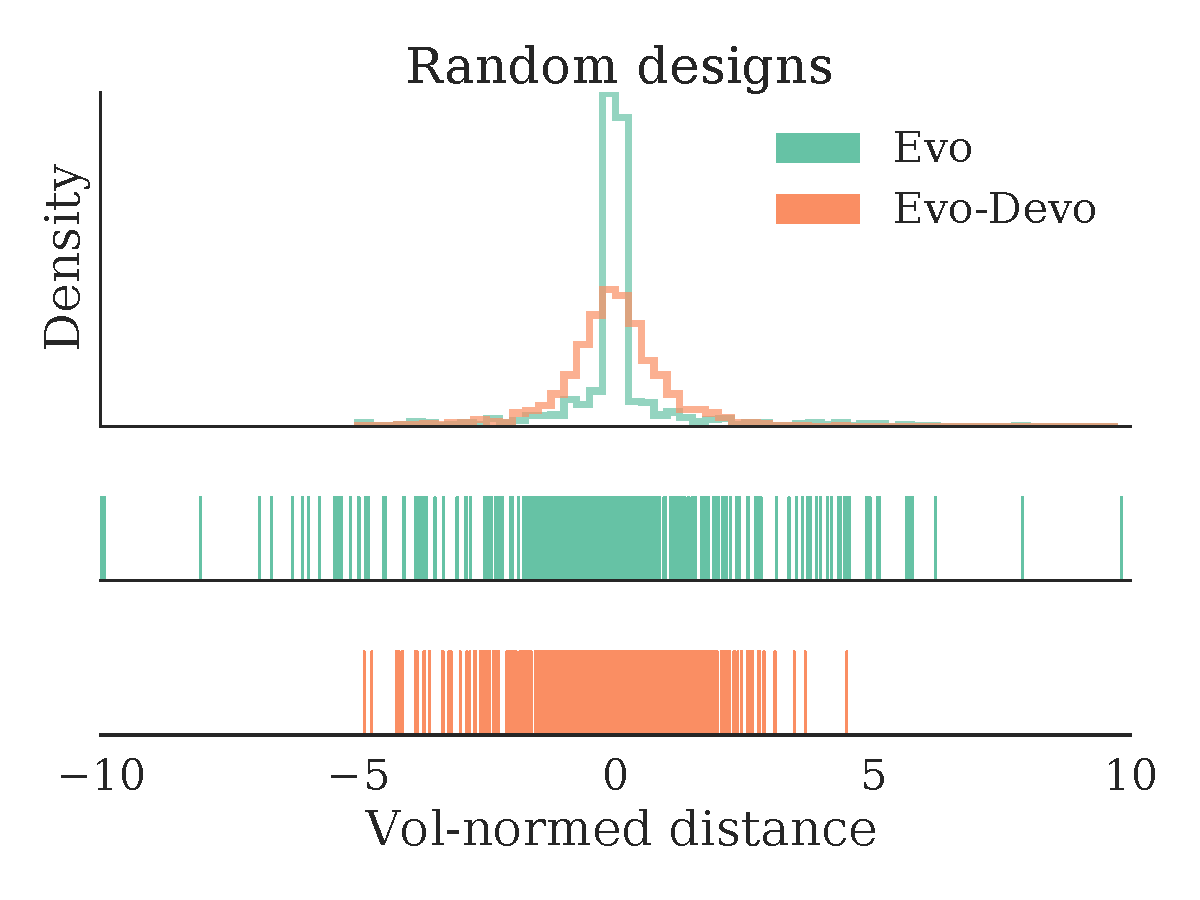
\includegraphics[width=0.6\textwidth]{Chapter03/img/random_distributions_gecco}
% \vspace{-0.6cm}
\caption{\label{fig:random} One thousand randomly generated robots for each group. 
The horizontal axes measure fitness: volume normalized distance in the positive $y$ direction.
The best overall designs are the best Evo robots since they maintain their good form as they behave. However, most designs are immobile (mode at zero) and Evo-Devo robots are more likely to move (less mass around zero) since they explore a continuum of body plans rather than a single static guess.}
\end{figure}


To get a sense of the evolutionary search space, prior to optimization, we randomly generated one thousand robots from each group (figure \ref{fig:random}).
The horizontal axes of figure \ref{fig:random} measure the fitness (equation \ref{eq3:fitness}) of our randomly generated designs.
The top portion of this figure plots the histogram of relative frequencies, using equal bin sizes between groups.
The mode is zero for both groups, meaning that the majority of designs are immobile.

The best possibility here is to randomly guess a good Evo robot since this good morphology is utilized for the full 32 actuation cycles. 
This is why the best random designs are Evo robots.
However, the Evo-Devo distribution contains much less mass around zero than the Evo distribution. It follows that it is more likely that an Evo-Devo robot moves at all, if only temporarily, since this only requires some interval of the many morphologies it sweeps over to be mobile. 
Also note that while the total displacement may be lower in the Evo-Devo case, since these robots `travel' through a number of different morphologies, they may pass through those which run at a higher instantaneous speed (but spend less of their lifetime in this morphology).



% nac: reword second sentence, awk

% nac: also note that while the total displacement may be lower in the Evo-Devo case, since the robots "travel" through a number of different morphologies, they may pass through those which travel at a higher instantaneous speed (but spend less of their lifetime in this morphology).  


\subsection*{Evolution.}

\begin{figure}[t]
\centering
% \hspace{-0.2cm}
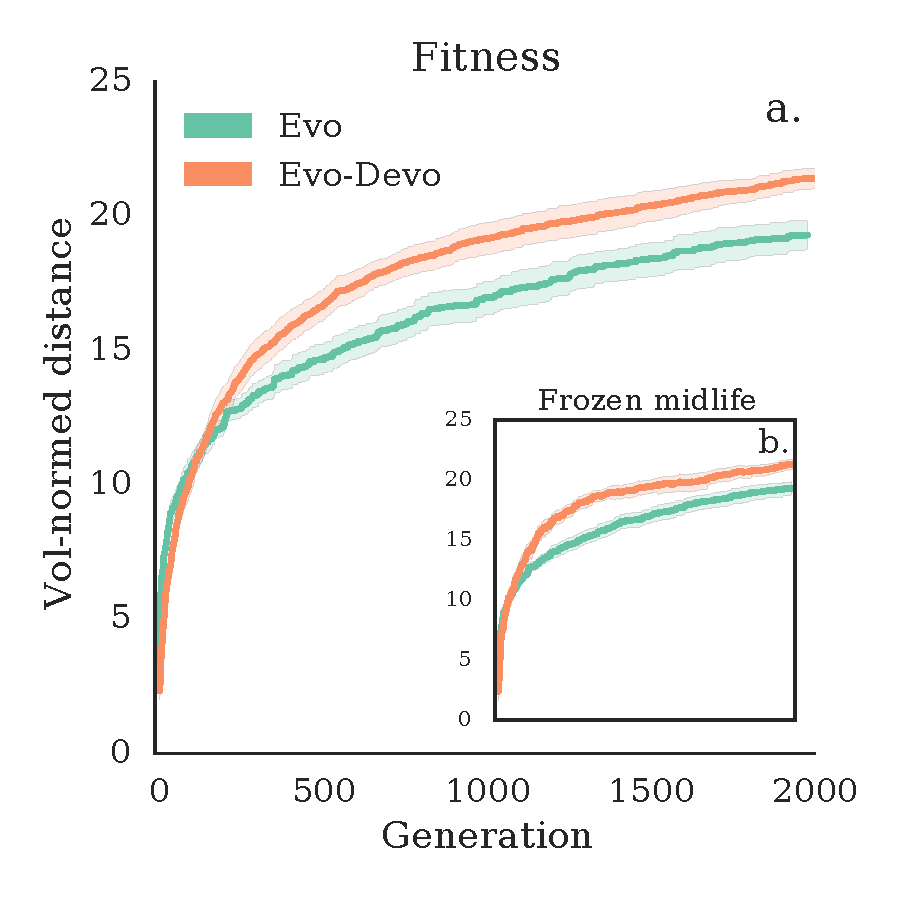
\includegraphics[width=0.6\textwidth]{Chapter03/img/main_frozen_gecco}
% \vspace{-0.7cm}
\caption{\label{fig:main_frozen} For thirty runs, a population of thirty robots is evolved for two thousand generations. (a) Best of generation fitness for Evo and Evo-Devo robots. (b) The same robots are reevaluated with development frozen at their midlife morphology.
Means are plotted with 95\% bootstrapped confidence intervals.}
\end{figure}


The results of the evolutionary algorithm are displayed in figure \ref{fig:main_frozen}a. 
In the earliest generations, evolution is consistent with random search and the best Evo robots start off slightly better than the best Evo-Devo robots.
However, the best Evo-Devo robots quickly overtake the best Evo robots. 
At the end of optimization there is a significant difference between Evo and Evo-Devo run champions ($U=122, \; p<0.001$).



We also chose to reevaluate Evo-Devo robots with their development frozen at their median ontogenetic morphologies (figure \ref{fig:main_frozen}b). For each robot, we measure the robot's fitness (equation \ref{eq3:fitness}) at this midlife morphology with development frozen, for two seconds. Selection is completely blind to this frozen evaluation. It exists solely for the purpose of post-evolution analysis, and serves primarily as a sanity check to make sure Evo-Devo robots are not explicitly utilizing their ability to grow/shrink to move faster.

Development appears to inhibit locomotion to some degree as the best morphologies run slightly faster with development turned off, particularly in earlier generations.
A significant difference, at the 0.001 level, between Evo robots and Evo-Devo robots with development frozen at midlife, occurs after only 108 generations compared to 255 generations with development enabled.
Note that the midlife morphology is not necessarily the top speed of an Evo-Devo robot. In fact it is almost certainly not the optimal ontogenetic form since the best body plan may occur at any point in its continuous ontogeny, including the start and endpoints.

% nac: "This does not appear to be the case" is vague, please clarify with example rather than implying knowledge with "This" -- especially across paragraphs



\subsection*{Closing the window.}

\begin{figure}[t]
% \hspace{-0.2cm}
\centering
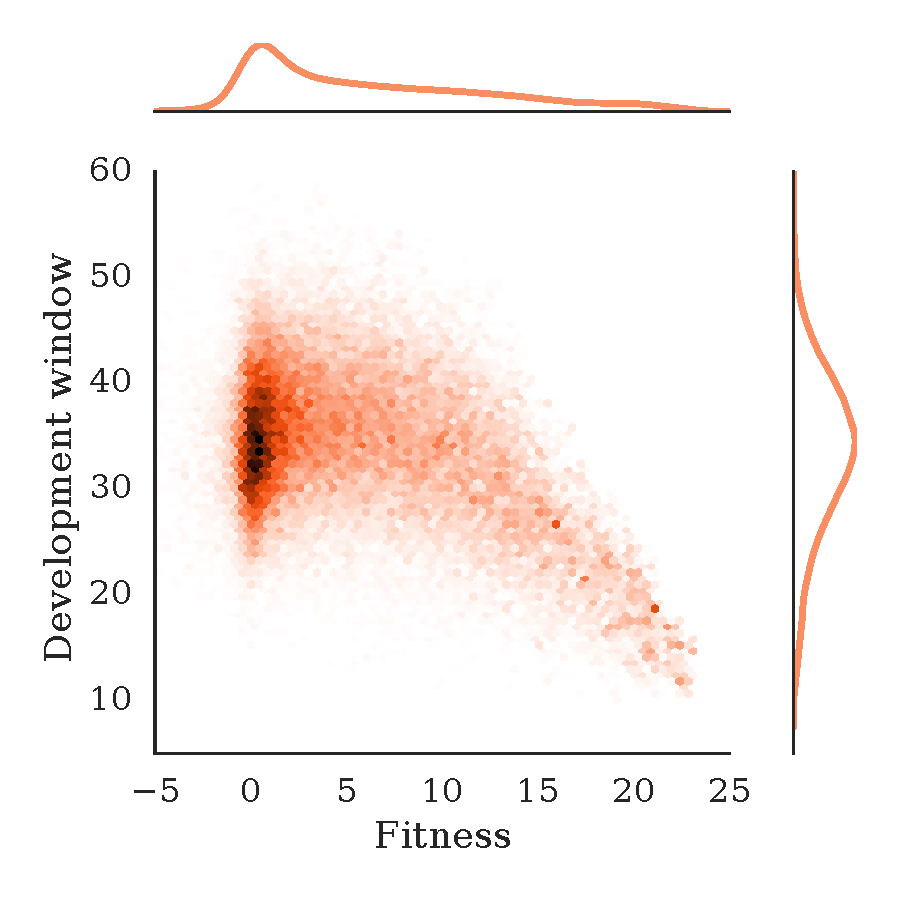
\includegraphics[width=0.6\textwidth]{Chapter03/img/window_gecco}
% \vspace{-0.7cm}
\caption{\label{fig:window} The relationship between the amount of development at the individual level ($W$) and fitness ($F$). The fastest individuals have small developmental windows surrounding a fast body plan.}
\end{figure}

\begin{figure}[t]
% \hspace{-0.2cm}
\centering
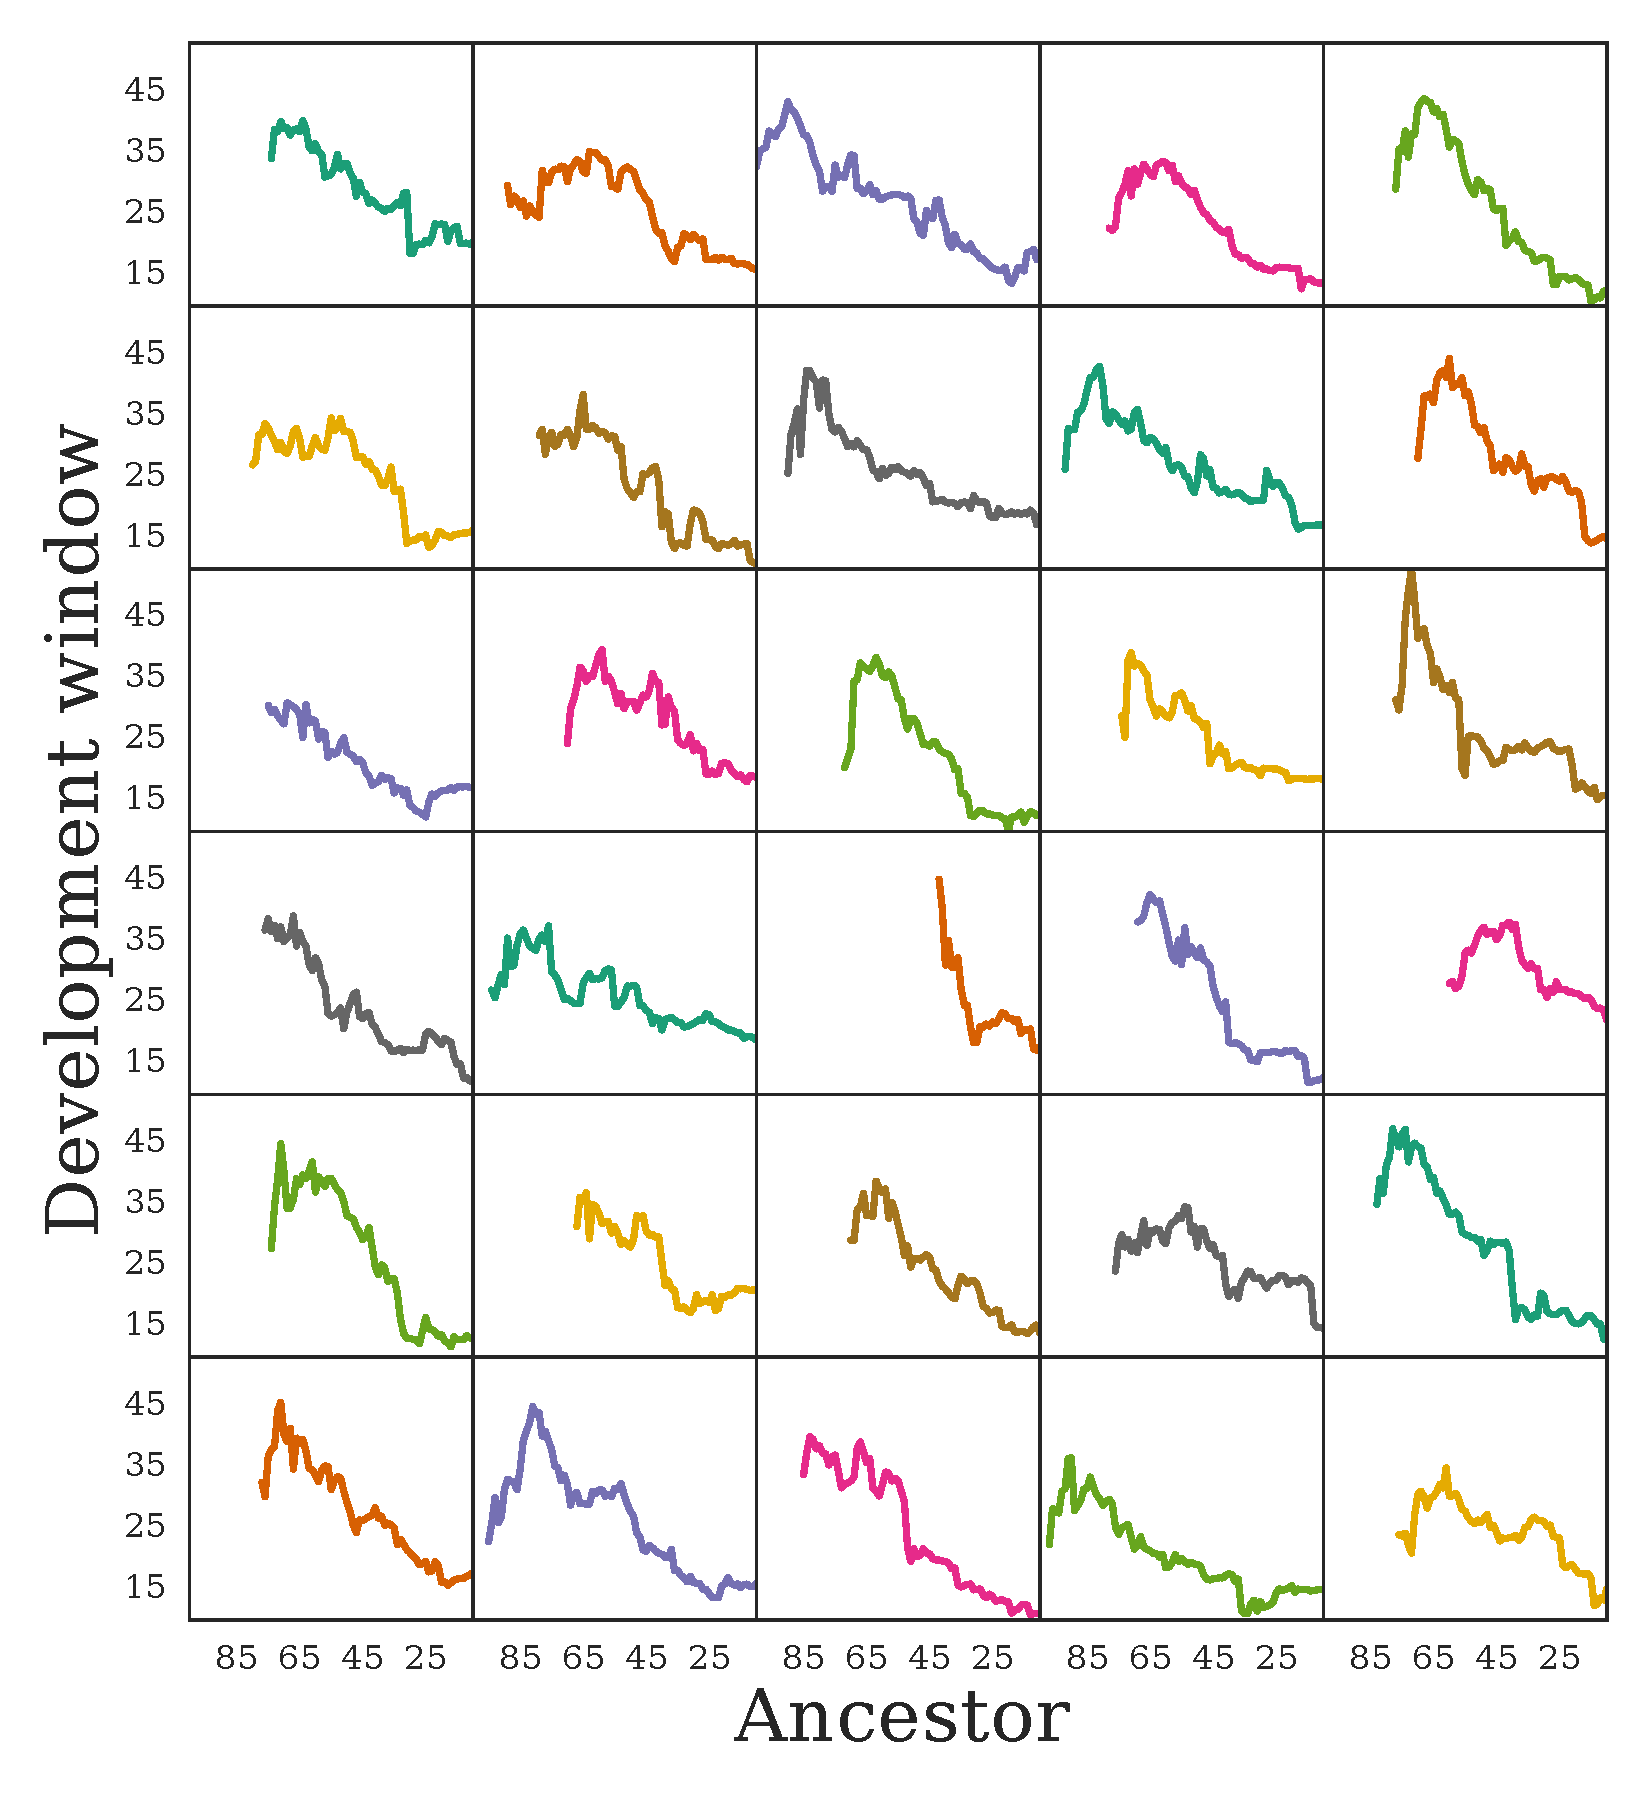
\includegraphics[width=0.65\textwidth]{Chapter03/img/ancestral_window_gecco}
% \vspace{-0.7cm}
\caption{\label{fig:ancestral_window} Closing the window. Total development window trajectories (in phylogeny) of the lineages of the most fit individuals in each run. Phylogenetic time goes from left to right: from the oldest ancestor (randomly created) to its most recent decedent, the current run champion.}
\end{figure}

Once an Evo-Devo robot identifies a good body plan in its ontogenetic sweep, its descendants can gain fitness by `suppressing' development around the good plan through heterochronic mutations.
This can be accomplished by incrementally closing the \textit{developmental window}, the interval $(s_{k0},\; s_{k1})$, for each voxel, around the good morphology.
In the limit, under a fixed environment, this process ends with a decedent born with the good design from the start and devoid of any developmental at all ($s_{k0} = s_{k1}$ for all voxels).
This phenomenon, best known as the Baldwin Effect, is instrumental in evolution
because natural selection is a hill-climbing process and therefore blind to needles in a haystack, good designs (local optima) to which no gradient of increased fitness leads.
The developmental sweep, however, alters the search space in which evolution operates, surrounding the good design
by a slope which natural selection can climb \cite{hinton1987learning}.


To investigate the relationship between development and fitness, we add up all of the voxel-level development windows to form a individual-level summary statistic, $W$. We define the \textit{total} development window, $W$, as the sum of the absolute difference of starting and final resting lengths across the robot's 48 voxels. 
\begin{equation}
W = \sum_{k=1}^{48} \text{abs}(s_{k1}-s_{k0})
\end{equation}

Overall there is a strong negative correlation between fitness, $F$, and the total development window, $W$, in Evo-Devo robots (figure \ref{fig:window}). 
To achieve the highest fitness values a robot needs to have narrow developmental windows at the voxel level.
However, this statistic doesn't discriminate between open/closed windows early/late in evolution. 
To show what sorts of development window/evolutionary time relationships eventually lead to highly fit individuals, we grab the lineages of only the most fit individuals at the end of evolutionary time (figure \ref{fig:ancestral_window}). 
In the most fit individuals, development windows tend to first increase slightly in phylogeny before decreasing to their minimum, or close nearby.
The age objective in AFPO lowers the selection pressure on younger individuals which allows them to explore, through larger developmental windows, a larger portion of design space until someone in the population discovers a locally optimal solution which creates a new selection pressure for descendants with older genetic material to `lock in' or canalize this form with smaller developmental windows.
These results further suggests that development itself is not optimal,
it is only helpful in that it can lead to better optima down the road once the window is closed.








\subsection*{The effect of mutations.}

\begin{figure*}
\centering
% \hspace{-0.85cm}
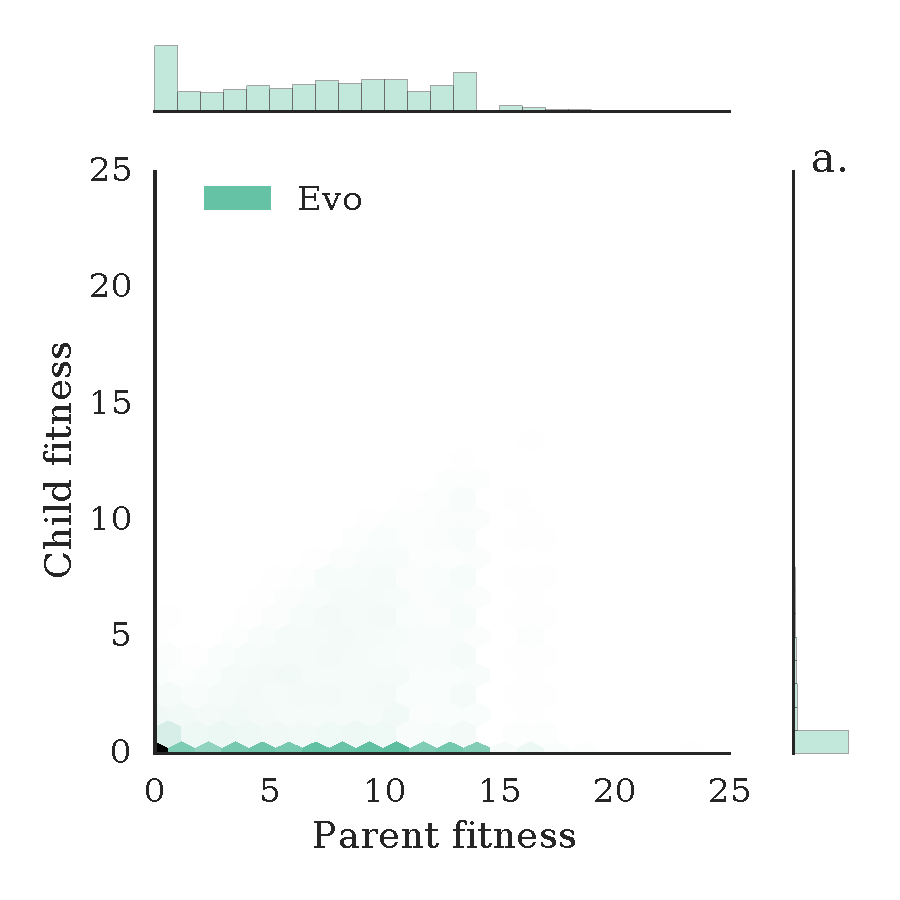
\includegraphics[width=0.495\textwidth]{Chapter03/img/mutations_gecco_evo_None}
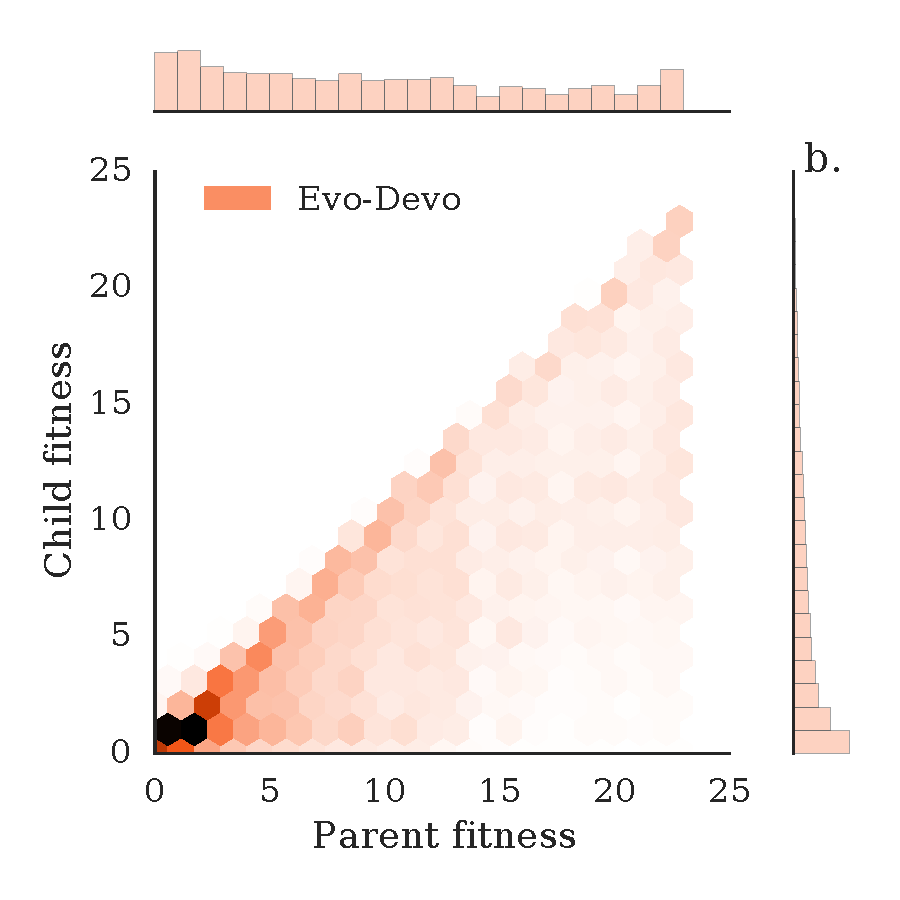
\includegraphics[width=0.495\textwidth]{Chapter03/img/mutations_gecco_devo_None}
% \vspace{-0.5cm}
\caption{\label{fig:mutations} Mutation impact: child fitness by parent fitness (vol-normed distance). The diagonal represents a neutral mutation, equivalent child and parent fitness. Hexagon bins below the diagonal represent detrimental mutations (child less fit than its parent); bins above the diagonal represent beneficial mutations (child more fit than its parent).}
\end{figure*}

% \begin{figure*}
% % \centering
% % \hspace{-0.85cm}
% 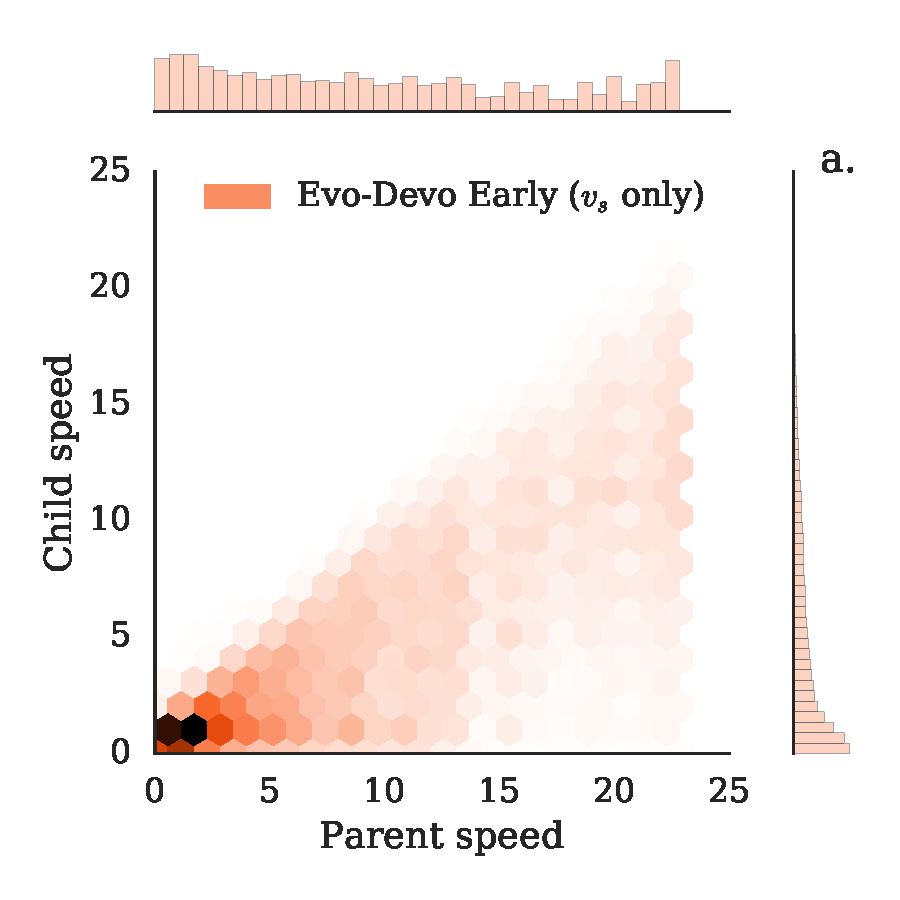
\includegraphics[width=0.495\textwidth]{Chapter03/img/mutations_gecco_devo_initial}
% 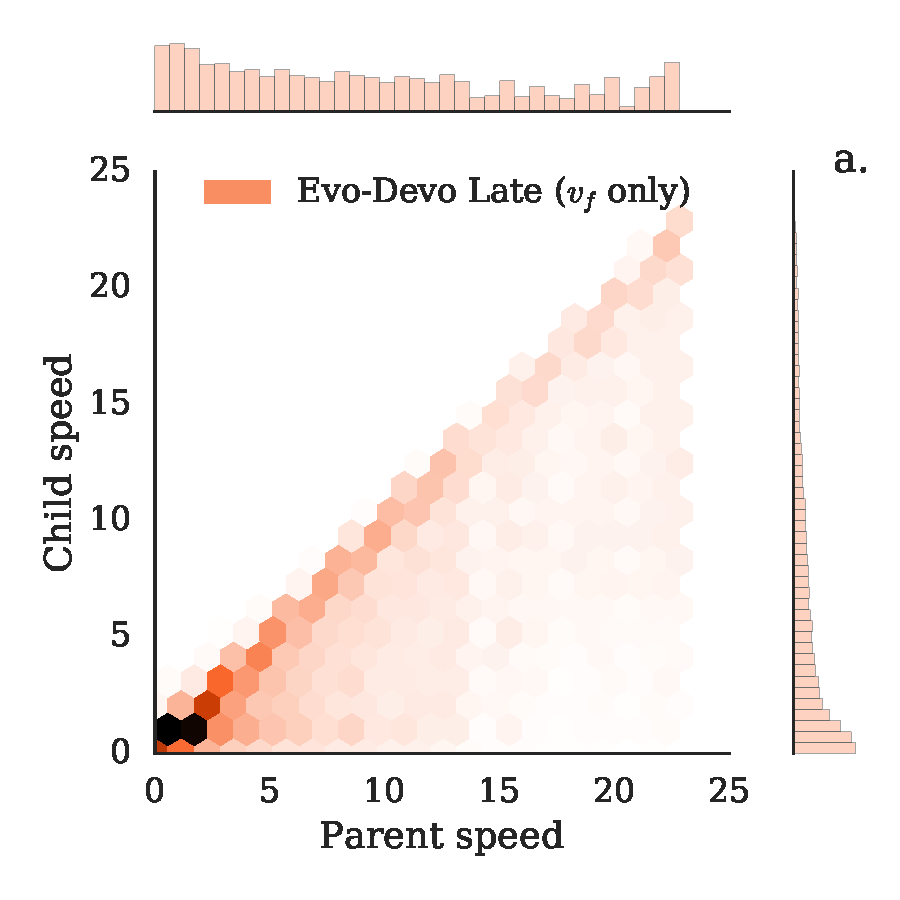
\includegraphics[width=0.495\textwidth]{Chapter03/img/mutations_gecco_devo_final}
% \vspace{-0.5cm}
% \caption{\label{fig:early_vs_late} {\color{red} These were not included for review. Is there a better way to illustrate this?  } Early vs late mutations.}
% \end{figure*}

In addition to the parameter-sweeping nature of its search,
developmental time provides evolution with a 
simple mechanism for inducing mutations with a range of magnitude
of phenotypic impact.
The overall mutation impact in our experiments is conveyed in figure \ref{fig:mutations} through 2D histograms of child and parent fitness. Recall that a child is created through mutation by each individual (parent) in the current population. These plots include the entire evolutionary history of all robots in every run. There are relatively so few robots with negative fitness that the histograms need not extend into this region since they contain practically zero density and would appear completely white.

The diagonal represents equal parent and child fitness, a behaviorally neutral mutation. Hexagons below the diagonal represent detrimental mutations: lower child fitness relative to that of its parent. Hexagons above the diagonal represent beneficial mutations: higher child fitness relative to that of its parent.
Mutations are generally detrimental for both groups, particularly in later generations once evolution has found a working solution.
For Evo robots (figure \ref{fig:mutations}a),
most if not all of the mass in the marginal density of child speed is concentrated around zero.
This means that mutations to an Evo robot are almost certain to break the existing parent solution, rendering a previously mobile design immobile.

The majority of Evo-Devo children, however, are generally concentrated on, or just below the diagonal in figure \ref{fig:mutations}b. 
This general pattern holds even in later generations when evolution has found working solutions with high fitness.
It follows that mutations to an Evo-Devo robot may be phenotypically smaller than mutations to an Evo robot, even though they use the same mutation operator. 
Furthermore, figure \ref{fig:mutations}b displays a high frequency of mutations with a wide range of magnitude of phenotypic impact including smaller, low-risk mutations which are useful for refining mobile designs; as well as a range of larger, higher-risk mutations which occasionally provide the high-reward of jumping into the neighborhood of a more fit local optima at a range of distances in the fitness landscape.


Now let's define the impact of developmental mutations, $M$, as the relative difference in child ($F_C$) and parent fitnesses ($F_P$), for positive fitnesses only.
\begin{equation}
M = \frac{F_C }{F_P}-1; \qquad F_C, \; F_P>0
\end{equation}
Then the average mutational impact for early-in-the-life mutations (any mutations that, at least in part, modify initial volumes) is $M_0=-0.29$.
While the average mutational impact for late-in-the-life mutations (that modify final volumes) is $M_1=-0.10$.
Although both types of mutations are detrimental on average, later-in-life mutations are more beneficial (less detrimental) on average ($p<0.001$).
This makes sense in a task with dependent time steps since a child created through a late-in-life mutation will at least start out with the same behavior as its parent and then slowly diverge over its life. Whereas an early-in-life mutation creates a behavioral change at $t=0$.

% nac: This intperpretation crucially assumes that time steps are not independent, and that changes early in life will affect other time steps later in life -- which change late in life cannot affect other times steps earlier in life.  



% \subsection*{Evolved morphologies and behaviors.}

% A robot can move a greater raw distance with a larger body. Not just because a single `footstep' is taken with a longer `leg', but also because the actuation is dampened for smaller volumes. Recall that a voxel at the minimum volume doesn't actuate at all to prevent simulation instability. This is in part why we chose our particular fitness function (equation \ref{eq3:fitness}) that normalizes distance by volume. As a result, the best performing individuals must efficiently utilize larger volumes in a trade off with speed analogous to energy preservation in nature. 

% Under our particular settings, `pinching in' internal voxel volumes is a common design element among evolved individuals.
% This creates a gap between hind and foreleg(s) which reduces volume while maintaining a fast body plan that walks in a straight line.
% The most fit individuals of each run tended to be either tripeds or quadrupeds, although this really depends on the definition of what constitutes a leg and how pronounced it must be. Many designs could be considered to be quadrupeds to some extent.
% Others clearly had a single front leg and/or a single back leg that was either flat or pointed at the center.
% The evolutionary history in figure \ref{fig:videos}, for example, started with no legs $(T=0)$, then three $(T=24)$ and finally four legs $(T>47)$. The particular ontogenetic timeline expanded in this figure (at $T=47$) starts with four legs but combines its hind legs into a single flat `foot' in ontogeny. 

% In terms of evolved behavior, gaits produced by uniform volumetric contraction/expansion tended to be less dynamic than previous work which evolved the placement of different patches of phase offset (`muscle') \cite{Cheney:2013:UEE:2463372.2463404} or more complex controllers with propagating waves \cite{cheney2014evolved}.
% Still, we found a few interesting gaits including the  alternating front-to-back kicking behavior depicted in figure \ref{fig:videos}.



\subsection*{The necessity of development.}

\begin{figure}
% \hspace{-0.2cm}
\centering
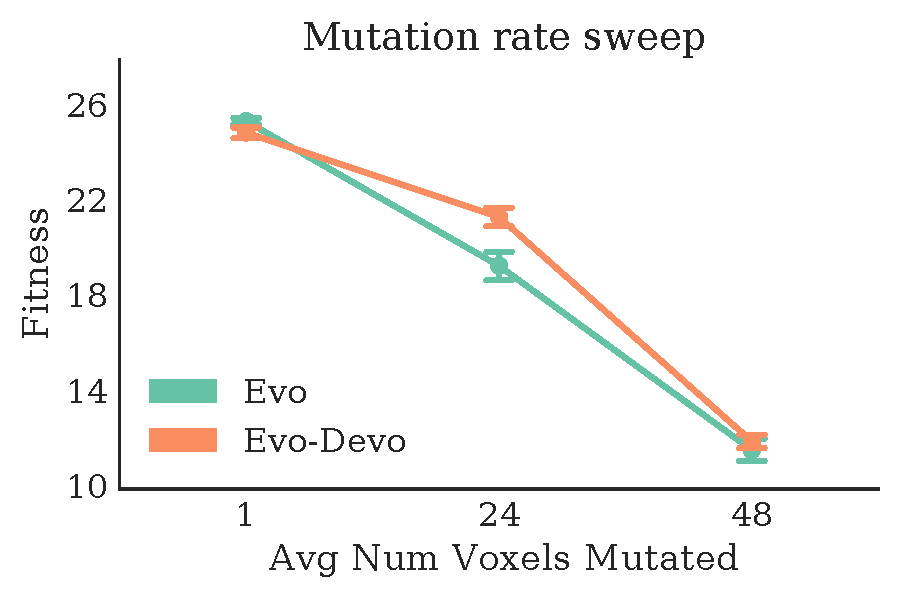
\includegraphics[width=0.6\textwidth]{Chapter03/img/sweep_gecco}
% \vspace{-0.7cm}
\caption{\label{fig:hyperparam_sweep} A hyperparameter sweep of mutation rate: a probability dictating the average number of voxels mutated in an individual robot.}
\end{figure}


In attempting to induce a needle-in-the-haystack fitness landscape, as a proof of concept, we intentionally set the mutation rate and scale fairly high.
A low-resolution hyperparameter sweep (figure \ref{fig:hyperparam_sweep}) indicates that the efficacy of ballistic development is indeed dependent on the mutation rate: there is no significant difference between Evo and Evo-Devo at either very low or very high rates. 
Higher fitness values are obtained through smaller mutation rates, which raises the question: Is development useful only in its ability to decrease the phenotypic impact of mutations?
If so we might prefer Evo robots (with a low mutation rate) since they reside in a smaller search space. 
But how low should the mutation rate be? 
It may in fact be difficult to know \textit{a priori} which mutation rate is optimal.
% We could in principle mutate Evo robots through specialized operators with a range of phenotypic impact.
It is also important to recognize that while we use mutation rate here to artificially tune the ruggedness of the fitness landscape, in a naturally rugged landscape we presumably would not have direct access to such an easily tunable parameter to `undo', or smooth-out the ruggedness.


Moreover, we know that there exist contexts in which developmental flexibility can permit the local speeding up of the basic, slow process of natural selection, thanks to the Baldwin Effect \cite{dennett2003baldwin}. 
Our new data suggests that even open-loop morphological change increases the probability of randomly finding (and subsequently `locking in') a mobile design (figure \ref{fig:random}), and that this probability is increasing in the amount of change (figure \ref{fig:ancestral_window}) even though ballistic development and fitness are inversely correlated (figure \ref{fig:window}). 
The staticity of Evo robots prevents this local speed-up which can place them at a significant disadvantage in rugged fitness landscapes.




% nac: no discussion section?  it might be nice to talk more abstractly about our hypotheses (for me especially the one of creating a gradient in the landscape by casting a wide net -- i.e. wide developmental windows -- and lessening its size over evolutionary time)




% Development in effect optimizes in a similar fashion to simulated annealing with an automatically refined cooling schedule

% JMS: ``developmental flexibility can lead to the genetic determination of a character that, in earlier generations, had to be acquired afresh each generation''



